% !TEX root = ../DuvalPeyre-SparseSpikes.tex

\section{Vanishing Derivatives Pre-certificate}
\label{sec-vanishing}

We show in this section that, if the Non Degenerate Source Condition holds, the minimal norm certificate $\eta_0$ is characterized by its values on the support of $m_0$ and the fact that its derivative must vanish on the support of $m_0$. Thus, one may compute the minimal norm certificate simply by solving a linear system, without handling
    the cumbersome constraint $\normi{\eta_0} \leq 1$.

%%%%%%%%%%%%%%%%%%%%%%%%%%%%%%%%
\subsection{Dual Pre-certificates}
Loosely speaking, we call \textit{pre-certificate} any ``good candidate'' for a solution of \eqref{eq-extremal-constrained}.
Typically, a pre-certificate is built by solving a linear system (with possibly a condition on its norm).
The following pre-certificate appears naturally in our analysis.

\begin{defn}[Vanishing derivative pre-certificate]\label{defn-vanishing-der-certif}
The vanishing derivative pre-certificate associated with a measure $m_0 = m_{a_0,x_0}$ is $\etaV = \Phi^* \pV$ where
\begin{align}
	\pV =\uargmin{p \in L^2(\TT)}�\norm{p}_2
		\quad \text{subj. to} \quad \foralls 1\leq i\leq N,\quad
	\choice{
		 (\Phi^* p)(x_{0,i})=\sign(a_{0,i}), \\
		 (\Phi^* p)'(x_{0,i})=0.
	}
\label{eq-vanishing-der-certif}
\end{align}
\end{defn}
It is clear that if the Source Condition (see Definition~\ref{def-source-cdt}) holds, then $\pV$ exists (since Problem~\eqref{eq-vanishing-der-certif} is feasible).
Observe that, in general, $\etaV$ is not a certificate for $m_0$ since it does not satisfy the constraint $\|\etaV\|_\infty\leq 1$.
The following proposition gathers several facts about the vanishing derivative pre-certificate which show that it is indeed a good candidate for the minimal norm certificate.


\begin{prop}
Let $m_0=m_{a_0,x_0}=\sum_{i=1}^N a_{0,i} \delta_{x_{0,i}}$ be a discrete measure.
The following assertions hold.
\begin{itemize}
  \item Problem~\eqref{eq-vanishing-der-certif} is feasible and $\|\etaV\|_\infty\leq 1$ if and only if the Source Condition holds and $\etaV=\eta_0$.
  \item If Problem~\eqref{eq-vanishing-der-certif} is feasible and $\Ga_{x_0}$ has full rank, i.e. $\Ga_{x_0}^* \Ga_{x_0} \in \RR^{2N \times 2N}$ is invertible, then 
    	\eq{
		\etaV = \Phi^* \Ga_{x_0}^{+,*} 
		\begin{pmatrix}
			\sign(a_0) \\
			0
		\end{pmatrix}
		\qwhereq
		\Ga_{x_0}^{+,*} = \Ga_{x_0}(\Ga_{x_0}^* \Ga_{x_0})^{-1}.
	}
\item If $\Ga_{x_0}$ has full rank, then $m_0$ satisfies the Non Degenerate Source Condition if and only if Problem~\eqref{eq-vanishing-der-certif} is feasible and 
\begin{align*}
	&\foralls s \in \TT\setminus \{x_{0,1},\ldots x_{0,N}\}, \quad &|\etaV(s)| < 1, \\
	&\foralls i\in \{1,\ldots N\}, \quad &\etaV''(x_{0,i}) \neq 0.
\end{align*}
\end{itemize}
\label{prop-vanish-tools}
\end{prop}

The third assertion of Proposition~\ref{prop-vanish-tools} states that it is equivalent to check the Non Degenerate Source Condition on $\eta_0$ (Definition~\ref{def-ndsc}) or to check the same conditions on $\etaV$. In case those conditions hold, one even has $\etaV=\eta_0$ (first assertion). The main point of this equivalence is that the second assertion yields a practical expression to compute $\etaV$ which may be used in numerical experiments (see Section~\ref{sec-vanishing-application}).

\begin{proof} 
  For the first assertion, we observe that if Problem~\eqref{eq-vanishing-der-certif} is feasible (and thus $\pV$ exists) and $\|\etaV\|_\infty\leq 1$, then $\etaV\in \partial{\normTV{m_0}}$ and the Source Condition holds. Hence, $\|\pV\|_2\geq \|p_0\|_2$. On the other hand the minimal norm certificate $\eta_0$ must satisfy all the constraints of \eqref{eq-vanishing-der-certif},  thus the minimality of the norms of both $\etaV$ and $\eta_0$ implies that $\etaV=\eta_0$. The converse implication is obvious.

For the second assertion, Problem~\eqref{eq-vanishing-der-certif}�can be written as
\eq{
	\etaV =  \uargmin{ \eta = \Phi^* p } \norm{p}_2.
	\quad \text{subj. to} \quad
	\choice{
		\Phi_{x_0}^*p = \sign(a_0), \\
		\Phi_{x_0}'^*p = 0,
	}
}
which is a quadratic optimization problem in a Hilbert space with a finite number of affine equality constraints.
Moreover, the assumption that $\Ga_{x_0}$ has full rank implies that the constraints are qualified. Hence it can be solved by introducing Lagrange multipliers $u$ and $v$ for the constraints. One should therefore solve the following linear system to obtain the value of $p=\pV$
	\eq{
		\begin{pmatrix}
			\Id 		& \Phi_{x_0} 	& \Phi'_{x_0} \\
			\Phi_{x_0}^*	& 0 	&0 \\
			{\Phi'_{x_0}}^*	& 0 	&0 \\
		\end{pmatrix}
		\begin{pmatrix}
			p \\ u \\ v
		\end{pmatrix}
		=
		\begin{pmatrix}
			0 \\ s \\ 0
		\end{pmatrix}.
	}
	Solving for $(u, v)$ in these equations gives the result. 
  
 
  For the third assertion, if the Non Degenerate Source condition holds, we apply Theorem~\ref{thm-noise-robustness} which yields a $C^1$ path $\la \mapsto (\tilde{a}_\la,\tilde{x}_\la )$ of solutions of $\Pp_\la(y_0)$ (we consider the case $w=0$). Then from Proposition~\ref{prop-vanish-certif} below, we obtain that $\etaV$ is a valid certificate and $\etaV=\eta_0$, hence $\etaV$ is non-degenerate.
The converse implication is a straightforward consequence of the first assertion.
\end{proof}


%%%%%%%%%%%%%%%%%%%%%%%%%%%%%%%%%%%%%%%%%%%%%%%%%%%%%%%%%%%%%%%%%%%%%%%%%%%%
\subsection{Necessary condition for support recovery}

There is a priori no reason for the vanishing derivative pre-certificate $\etaV$ to satisfy
$\normi{\etaV}\leq 1$. Here, we prove that that is in fact a necessary condition for (noiseless) exact support recovery to hold on some interval $[0,\la_0)$ with $\la_0>0$, \textit{i.e.} the solutions of $\Pp_\la(y_0)$ having exactly $N$ spikes which converge smoothly towards those of the original measure.
 
\begin{prop}
Let $m_0=m_{a_0,x_0}=\sum_{i=1}^N a_{0,i} \delta_{x_{0,i}}$ be a discrete measure such that $\Ga_{x_0}$ has full rank. 
Assume that there exists $\la_0>0$ and a $C^1$ path $[0,\la_0)\rightarrow \RR^N\times \TT^N$, $\la \mapsto (a_\la, x_\la)$ such that for all $\la\in [0,\la_0)$ the measure $m_\la=m_{a_\la,x_\la}$ is a solution to $\Pp_\la(y_0)$ (the noiseless problem).
  
  Then $\etaV$ exists, $\|\etaV\|_\infty\leq 1$ and $\etaV=\eta_0$.
\label{prop-vanish-certif}
\end{prop}

\begin{proof}
  Let $p_\la =\frac{1}{\la} (y_0-\Phi m_\la)=\frac{1}{\la} (\Phi_{x_0}a_0 -\Phi_{x_\la} a_\la)$ be the certificate defined by the optimality conditions~\eqref{eq-extremal-cdt}. We show that $\Phi^* p_\la$ converges towards $ \Phi^* \Ga_{x_0}^{+,*} 
		\begin{pmatrix}
			\sign(a_0) \\
			0
		\end{pmatrix}=\etaV$
 (and that the latter exists).

Writing
	\eq{
    a_\la' = \frac{\d a_\la}{\d\la} \in \RR^N
		\qandq
		x_\la' = \frac{\d x_\la}{\d\la} \in \RR^N,
	}
 we observe that for any $i\in \{1,\ldots N\}$ and any $x\in \TT$, 
\begin{align*}
	&\frac{a_{\la,i}\varphi (x_{\la, i}-x) - a_{0,i}\varphi (x_{0, i}-x)}{\la}- \left[ a_{0,i}\varphi' ( x_{0, i}-x) x_{0,i}' + a_{0,i}'\varphi ( x_{0, i}-x) \right]\\
 &\quad = \int_{0}^1 \left[ a_{\la t,i}\varphi' ( x_{\la t, i}-x) x_{\la t,i}' + a_{\la t,i}'\varphi ( x_{\la t, i}-x) \right]\\
 & \qquad \qquad - \left[ a_{0,i}\varphi' ( x_{0, i}-x) x_{0,i}' + a_{0,i}'\varphi ( x_{0, i}-x) \right]  \d t,
\end{align*}
and the latter integral converges (uniformly in $x$) to zero when $\la \to 0^+$ by uniform continuity of its integrand (since $ a$, $ x$ and $\varphi$ are $C^1$).
As a consequence, we obtain that $\frac{y_0-\Phi_{ x_\la}{a}_\la}{\la}$ converges uniformly to $-\Ga_{x_0}
		\begin{pmatrix}
			\Id & 0 \\ 0 & \diag(a_0)
		\end{pmatrix}
		\begin{pmatrix}
			 a_0' \\  x_0'
		\end{pmatrix}$.

    On the other hand, we observe that for $\la$ small enough, $\sign (a_\la)=\sign (a_0)$, and using the notations of the proof of Theorem~\ref{thm-noise-robustness}, the implicit equation $E_{s_0}(a_\la,x_\la,\la,0)=0$ holds. Differentiating that equation at $\la=0$ we obtain:
\begin{align*}	
  \pa{ \pd{E_{s_0}}{(a,x)}(a_0,x_0,0,0) }
			\begin{pmatrix}
			 a_0' \\  x_0'
		\end{pmatrix}
	+\pd{E_{s_0}}{\la}(a_0,x_0,0,0)&=0, 
\end{align*}
or equivalently
\begin{align*}	
	(\Ga_{x_0}^* \Ga_{x_0})\begin{pmatrix}
		\Id & 0 \\ 0 & \diag(a_0)
	\end{pmatrix}
\begin{pmatrix}
			 a_0' \\  x_0'
		\end{pmatrix}
&= - 	\begin{pmatrix}
		s_0\\
		0
	\end{pmatrix}.
\end{align*}

As a consequence, Problem~\eqref{eq-vanishing-der-certif} is feasible and we see that $\frac{y_0-\Phi_{ x_\la}{a}_\la}{\la}$ converges uniformly (and thus in the $L^2$ strong topology) to $\Ga_{x_0}(\Ga_{x_0}^* \Ga_{x_0})^{-1}\begin{pmatrix}
			\sign(a_0) \\
			0
		\end{pmatrix}$ and $\Phi^*\left(\frac{y_0-\Phi_{ x_\la}}{\la}\right)$ converges uniformly to $\Phi^* \Ga_{x_0}^{+,*} 
		\begin{pmatrix}
			\sign(a_0) \\
			0
    \end{pmatrix}$ (which is precisely $\etaV$ from the second assertion of Proposition~\ref{prop-vanish-tools}).

   Since $\|\Phi^* \left(\frac{y_0-\Phi_{ x_\la}a_\la}{\la}\right)\|_\infty = \|\Phi^*p_\la\|_\infty\leq 1$ for all $\la >0$, we obtain that $\|\etaV\|_\infty\leq 1$, hence the claimed result.
\end{proof}


%%%%%%%%%%%%%%%%%%%%%%%%%%%%%%%%%%%%%%%%%%%%%%%%%%%%%%%%%%%%%%%%%%%%%%%%%%%%
\subsection{Application to the Ideal Low-pass Filter}
\label{sec-vanishing-application}

In order to prove their identifiability result for measures, the authors of~\cite{Candes-toward} also introduce a ``good candidate'' for a dual certificate associated with $m=m_{a,x}$ for $a \in \CC^N$ and $x \in \RR^N$. 
For $K$ being the square of the Fejer kernel, they build a trigonometric polynomial
\eq{
	\etaCF(t)=\sum_{i=1}^N \left(\alpha_{i}K(t-x_i) + \beta_{i}K'(t-x_i) \right) \mbox{ with } K(t)=\left(\frac{\sin \left(\left(\frac{f_c}{2}+1 \right)\pi t\right)}{\left(\frac{f_c}{2}+1\right)\sin \pi t}\right)^4
}
and compute $(\al_i,\be_i)_{i=1}^N$ by imposing that $\etaCF(x_i)=\sign (a_i)$ and $(\etaCF)' (x_i)=0$.

They show that the constructed pre-certificate is indeed a certificate,  i.e. that $\normi{\etaCF} \leq 1$, provided that the support is separated enough (i.e. when $\Delta(m)\geq C/f_c$). This result is important since it proves that measures that have sufficiently separated spikes are identifiable. Furthermore, using the fact that $\etaCF$ is not degenerate (i.e. $(\etaCF)''(x_i) \neq 0$ for all $i=1,\ldots,N$), the same authors derive  an $L^2$ robustness to noise result in~\cite{Candes-superresol-noisy}, and Fernandez-Granda and Azais et al.  use the constructed certificate to analyze finely the local averages of the spikes in~\cite{Fernandez-Granda-support,Azais-inaccurate}.

From a numerical perspective, we have investigated how this pre-certificate compares with the vanishing derivative pre-certificate that appears naturally in our analysis, by generating real-valued measures for different separation distances and observing  when each pre-certificate $\eta$ satisfies $\normi{\eta} \leq 1$.


%\begin{figure}[ht]
%\centering
%	\begin{tabular}{@{}c@{\hspace{1mm}}c@{}}
%	   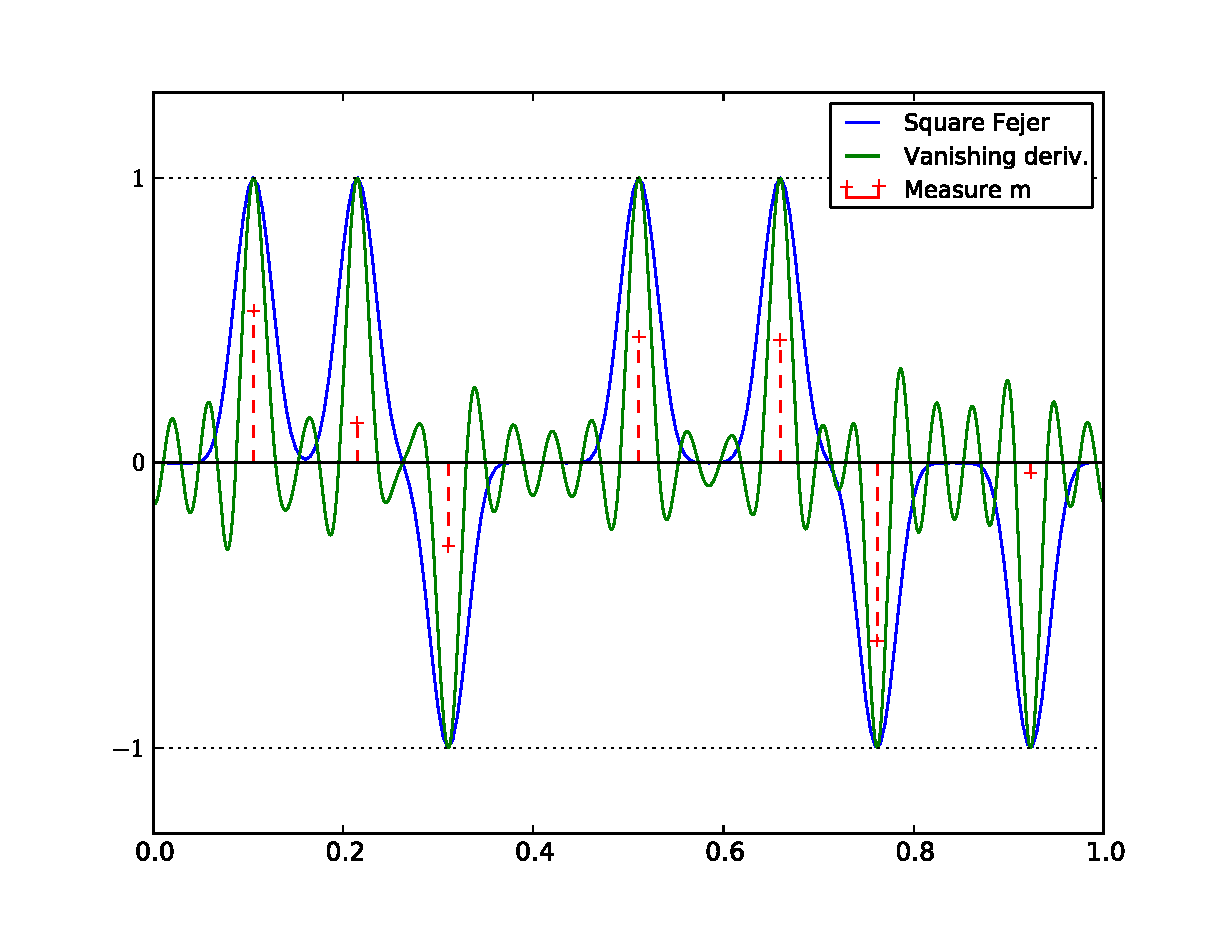
\includegraphics[width=0.46\linewidth] {precertif-2p5.pdf} &
%   		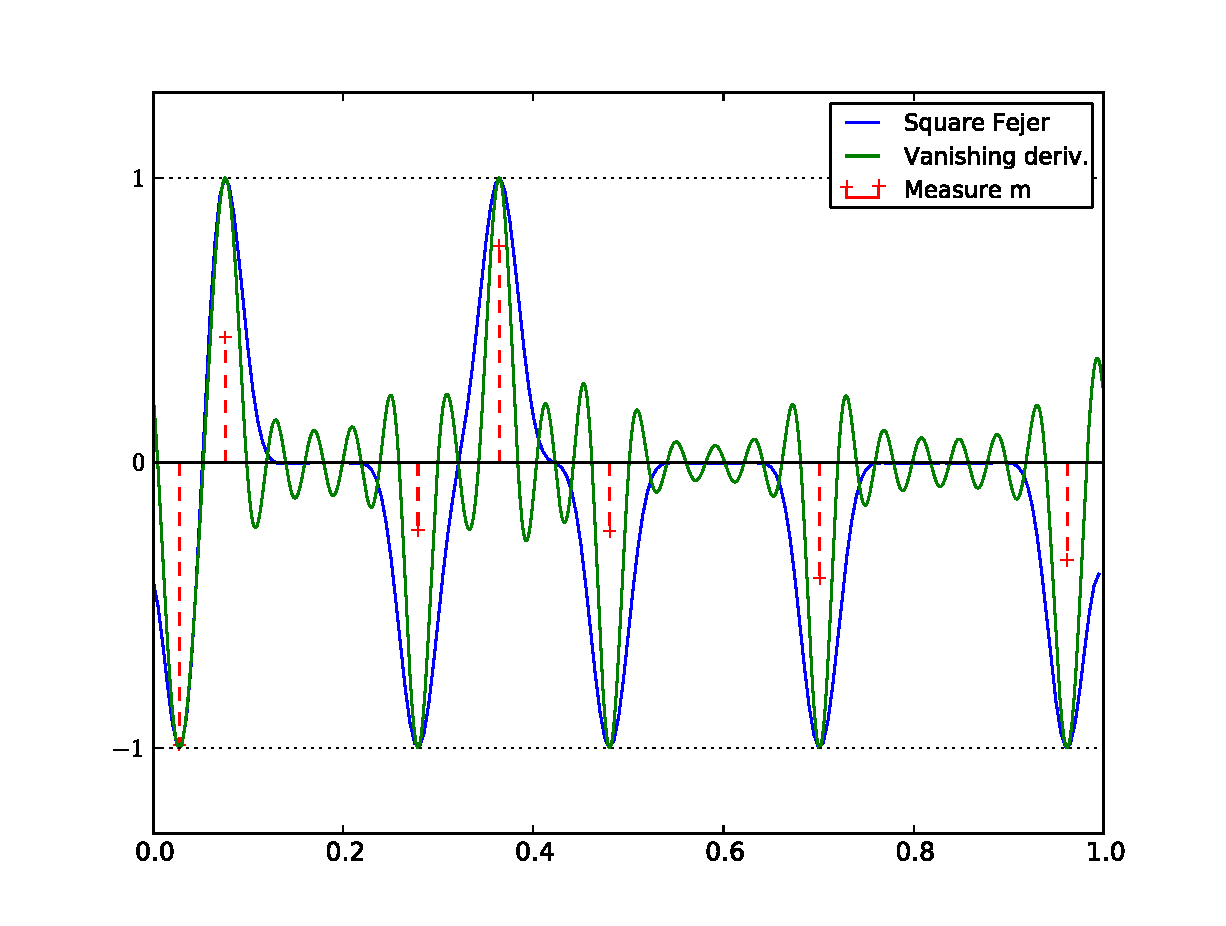
\includegraphics[width=0.46\linewidth] {precertif-1p26.pdf} \\
%		$\Delta(m)\approx 2.50/f_c$ & $\Delta(m)\approx 1.26/f_c$ \\[3mm]
%	   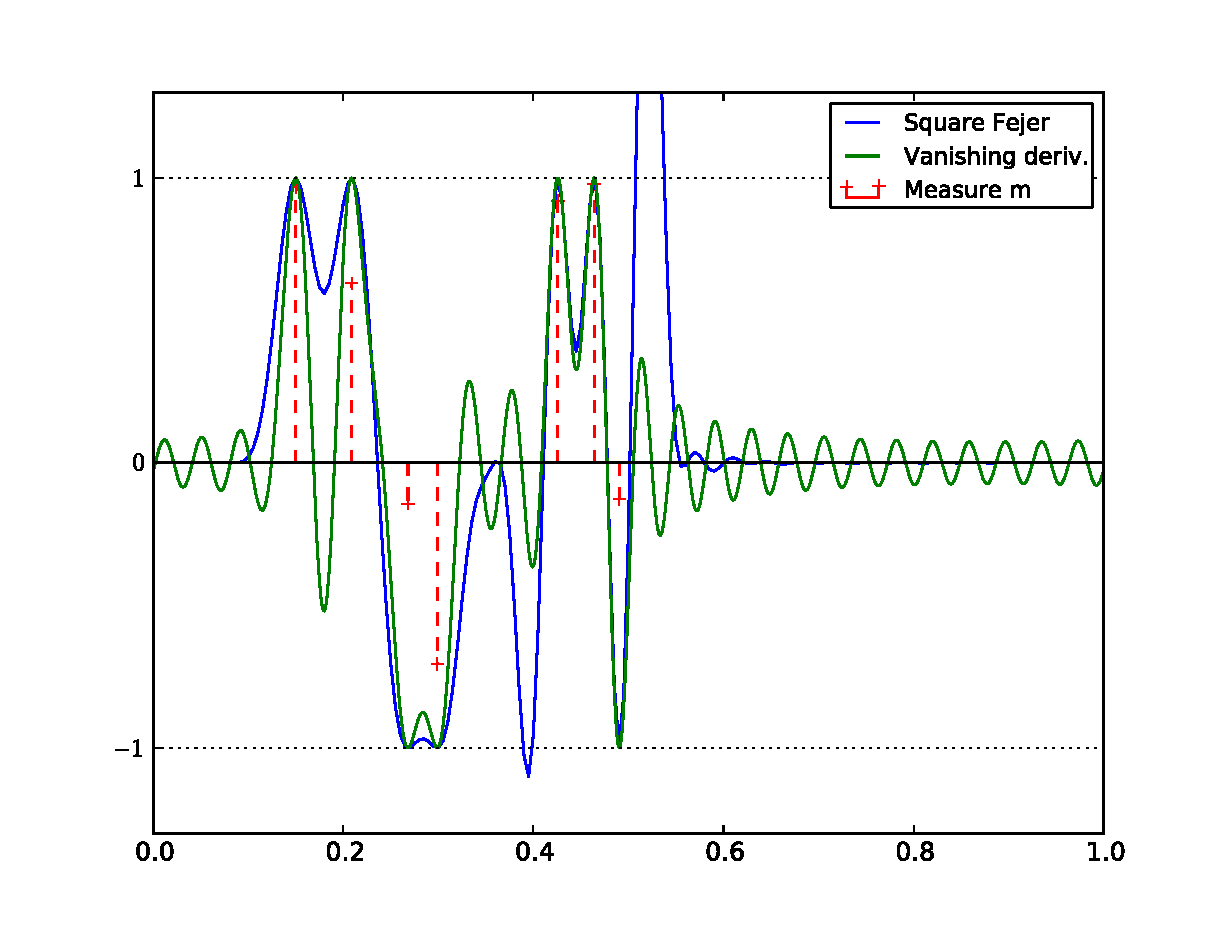
\includegraphics[width=0.46\linewidth] {precertif-0p69.pdf} &
%	   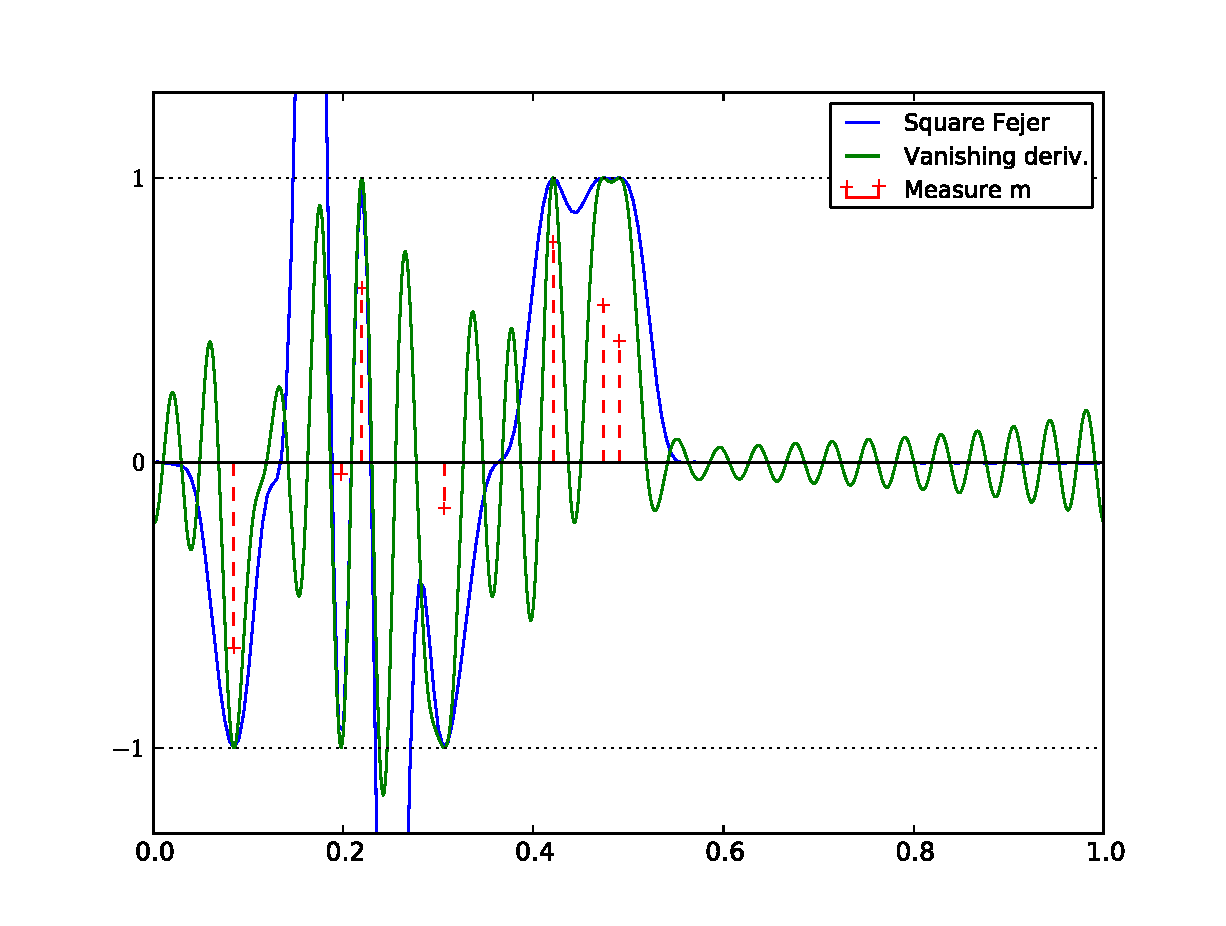
\includegraphics[width=0.46\linewidth] {precertif-0p44.pdf}\\
%		$\Delta(m)\approx 0.69/f_c$ & $\Delta(m)\approx 0.44/f_c$
%	\end{tabular}
%\caption{\label{fig-precertif} % 
%The blue curve is the square Fejer kernel pre-certificate $\hat \eta_0$ (introduced in~\cite{Candes-toward}) and the green curve shows the vanishing derivative pre-certificate $\bar\eta_0$, defined in~\eqref{eq-vanishing-der-certif}, for several measures $m$ (whose Diracs' locations and elevation are display in dashed red) with different separation distances $\De(m)$. Eventually when $\Delta(m)$ is small enough, both pre-certificates break (i.e. are not anymore certificates), but the square Fejer always breaks before the vanishing derivative pre-certificate.\vspace{2mm}}
%\end{figure}


\begin{figure}[ht]
\centering
% \begin{tabular}{@{}c@{}c@{}}
\subfloat[$\Delta(m_0)=0.8/f_c$]{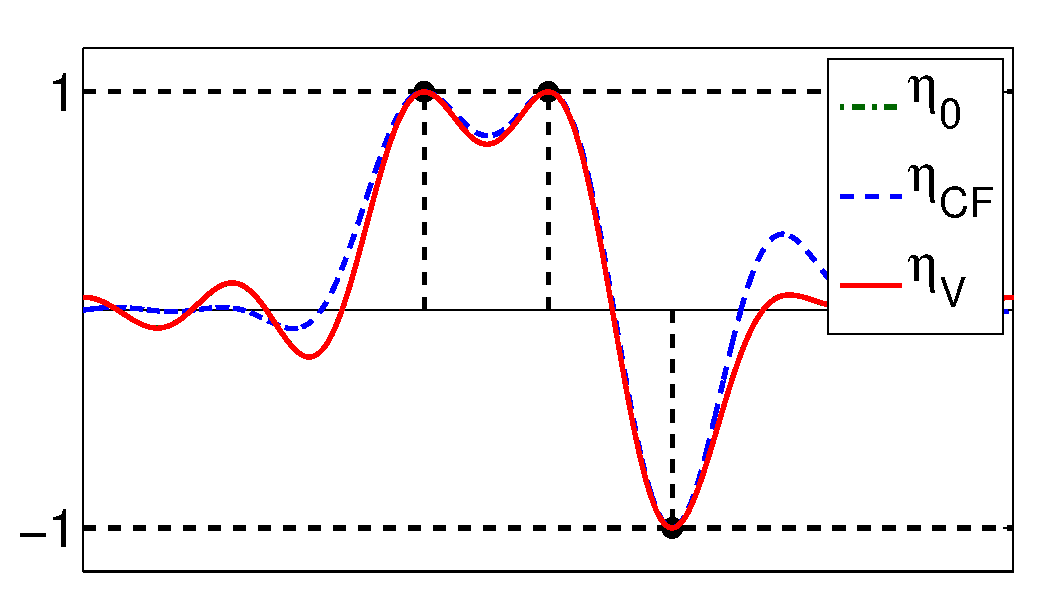
\includegraphics[width=0.49\linewidth]{certificates/ideal-3diracsa-80}}
\subfloat[$\Delta(m_0)=0.7/f_c$]{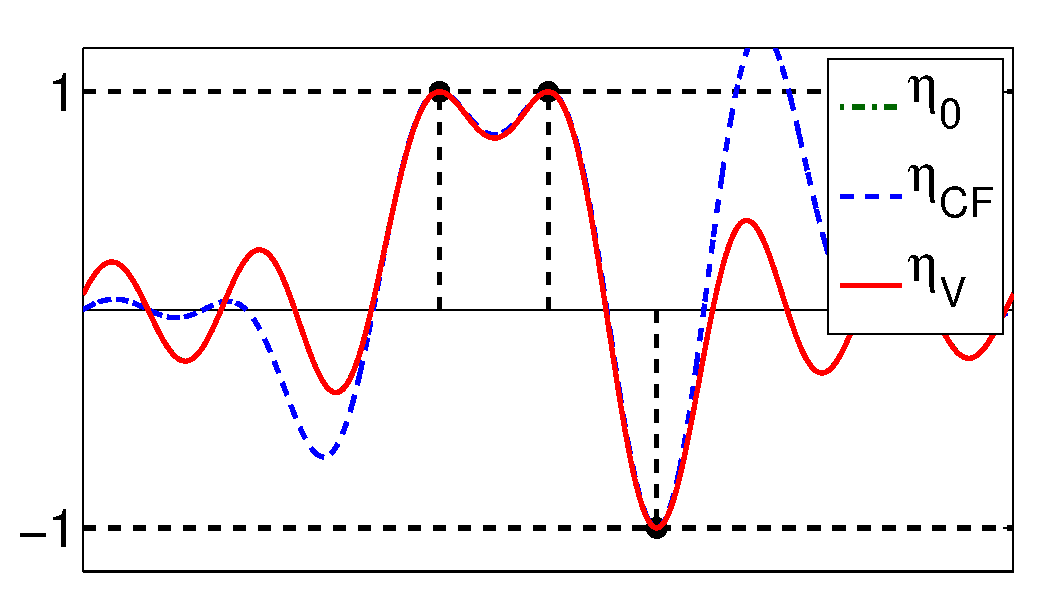
\includegraphics[width=0.49\linewidth]{certificates/ideal-3diracsa-70}}\\
\subfloat[$\Delta(m_0)=0.6/f_c$]{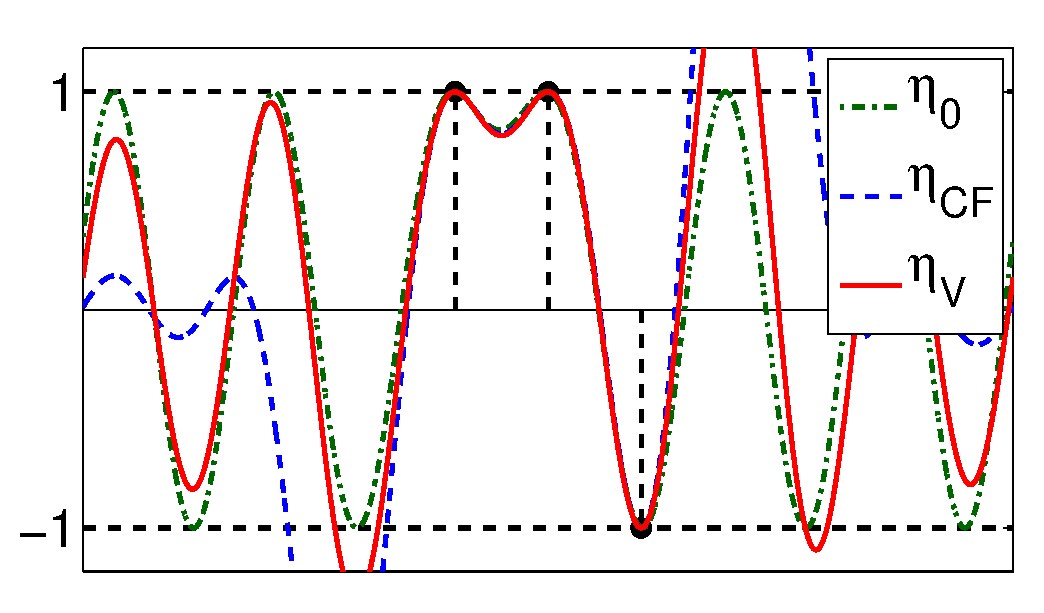
\includegraphics[width=0.49\linewidth]{certificates/ideal-3diracsa-60}}
\subfloat[$\Delta(m_0)=0.5/f_c$]{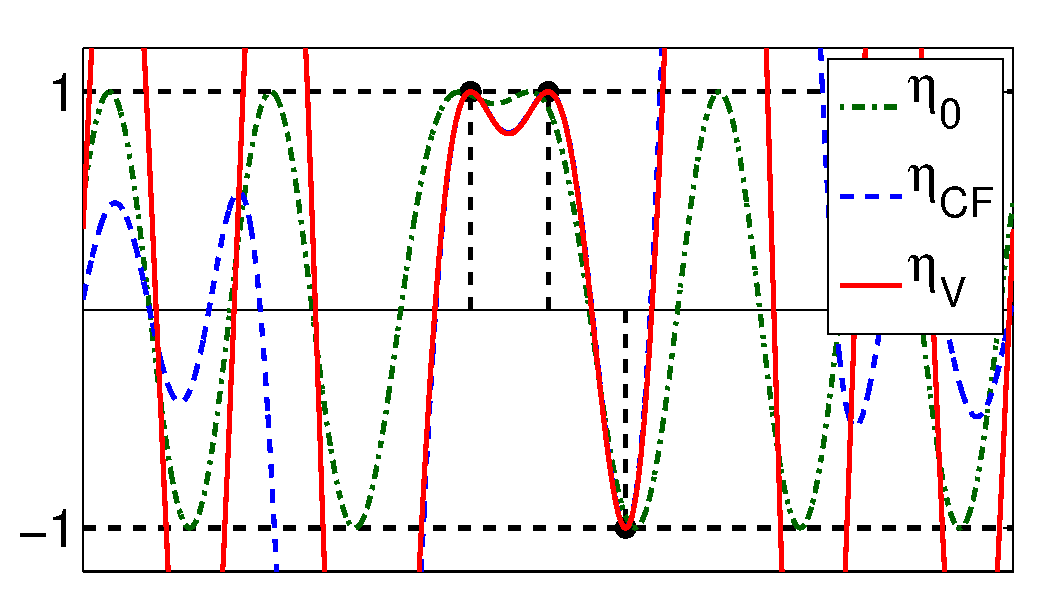
\includegraphics[width=0.49\linewidth]{certificates/ideal-3diracsa-50}}
\caption{\label{fig-certif} % 
Pre-certificates for three equally spaced masses. The blue curves with dots is the Fejer
 pre-certificate $\etaCF$, while red continuous line is the vanishing derivative $\etaV$. The 
 black dashed line is the minimal norm precertificate $\eta_0$.\vspace{2mm}}
\end{figure}


As predicted by the result of~\cite{Candes-toward}, we observe numerically that the pre-certificate
 $\etaCF$ is a certificate (i.e. $\normi{\etaCF} \leq 1$) for any measure with $\De(m_0) \geq 1.87/f_c$.
 We also observe that this continues to hold up to $\De(m_0) \geq 1/f_c$. Yet, below $1/f_c$,
 it may happen that some measures are still identifiable (as asserted using the
 vanishing derivative pre-certificate $\etaV$)  but $\etaCF$ stops being a certificate, i.e.
 $\normi{\etaCF} > 1$. A typical example is shown in Figure~\ref{fig-certif}, where, for $f_c=6$
 we have used three equally spaced masses as an input, their separation distance being
 $\Delta(m_0)\in \{\frac{0.8}{f_c},\frac{0.7}{f_c},\frac{0.6}{f_c},\frac{0.5}{f_c}\}$. 
 Here, we have computed an approximation of the minimal norm certificate $\eta_0$ by solving
  \eqref{eq-initial-dual} with very small $\la$.
 
 For $\Delta(m_0)=\frac{0.8}{f_c}$, both $\etaV$ and $\etaCF$ are certificates, so that the
vanishing derivatives pre-certificate $\etaV$ is equal to the minimal norm certificate $\eta_0$.
For $\Delta(m_0)=\frac{0.7}{f_c}$, $\etaCF$ violates the constraint $\normi{\etaCF}\leq 1$ but
 the vanishing derivative pre-certificates is still a certificate (even showing that the measure
is identifiable). For $\Delta(m_0)=\frac{0.6}{f_c}$ and $\frac{0.5}{f_c}$, neither $\etaV$ nor $\etaCF$
satisfy the constraint, hence $\etaV \neq \eta_0$. Yet, $\eta_0$ ensures that $m_0$ is a solution to \eqref{eq-constrained-pbm}.
 
  
 % Yet, below $1/f_c$,
% we observe numerically that some measures are still identifiable (as asserted using the
% vanishing derivative pre-certificate $\etaV$)  but $\etaCF$ stops being a certificate, i.e.
% $\normi{\etaCF} > 1$. An illustration is given in Figure~\ref{fig-precertif}, where the
%  chosen parameters are $f_c=26$ and $N=7$. For the cases $\Delta(m)=2.50/f_c$ and
%   $\Delta(m)=1.26/f_c$, both pre-certificates $\etaV$ and $\etaCF$ are certificates,
% showing that the generated measure is identifiable. Notice how the vanishing derivative
% certificate $\etaV$ oscillates much more than the square Fejer certificate $\etaCF$ . For
% $\Delta(m)=0.69/f_c$, the square Fejer pre-certificate breaks the constraint
%  ($\normi{\etaCF} \approx 2.39$) whereas the vanishing derivative certificate still satisfies
% $\normi{\etaV} \leq 1$. Eventually, for $\Delta(m)=0.44/f_c$, both pre-certificates violate
% the constraint, with $\normi{\etaCF} \approx 3.39$ and $\normi{\etaV}=1.17$.
% 


\begin{figure}[ht]
\centering
\subfloat[$m$ and certificates]{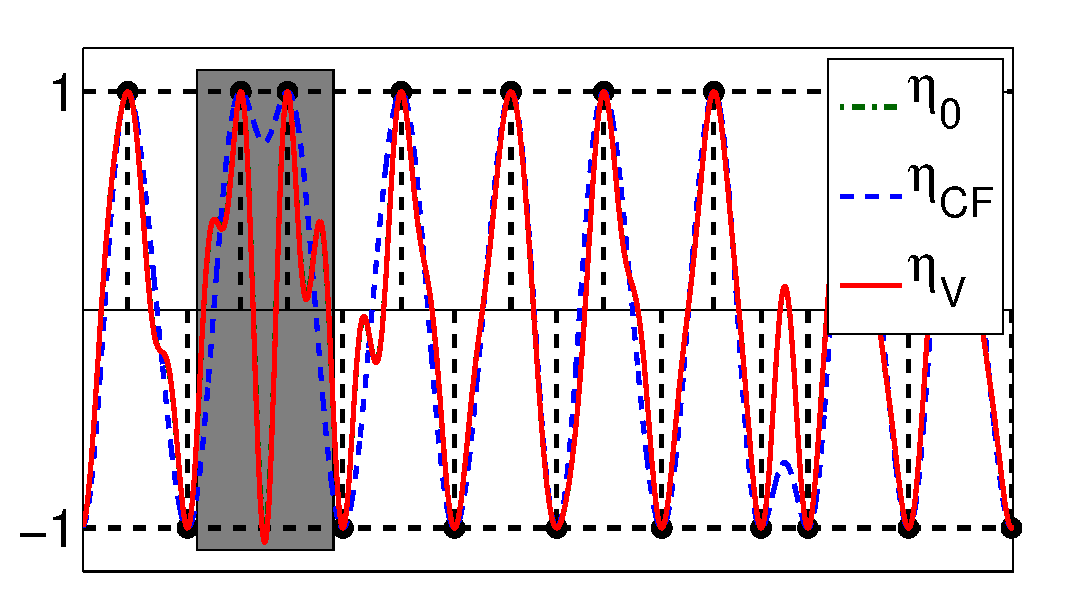
\includegraphics[width=0.49\linewidth]{certificates-pathological/ideal-pathological3-70}}
\subfloat[Zoom on the gray area]{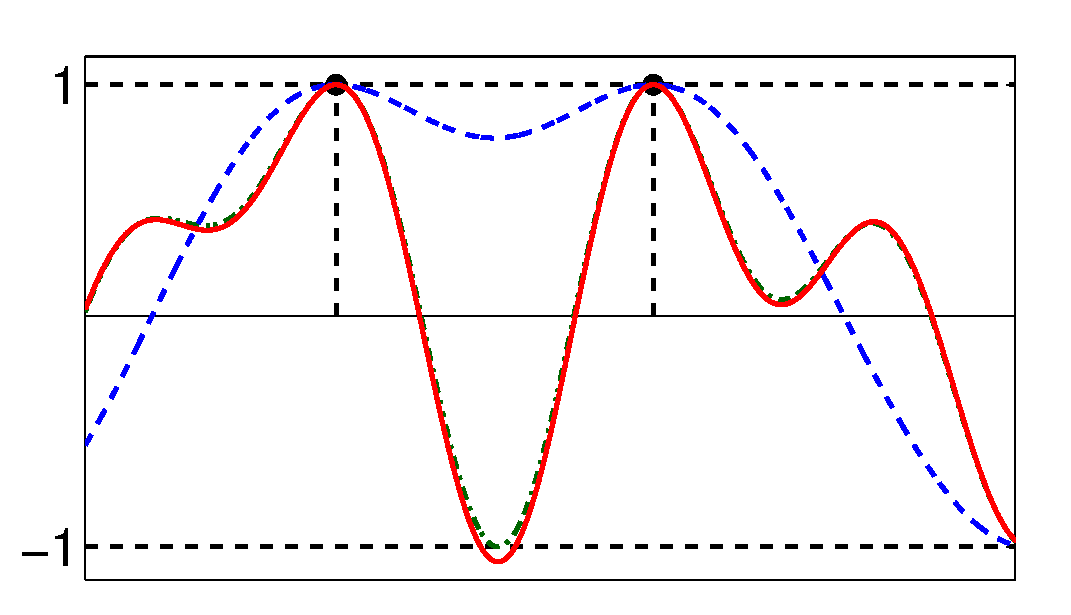
\includegraphics[width=0.49\linewidth]{certificates-pathological/ideal-pathological3-70-zoom}}
\caption{\label{fig-certif-pathologic} % 
	Example of measure for which $\etaV \neq \eta_0$. }
\end{figure}


From the experiments we have carried out, we have observed that the vanishing derivative pre-certificate $\etaV$
 behaves in general at least as well as the square Fejer $\etaCF$. The only exceptions we have 
noticed is for a large number of peaks (when $N$ is close to $f_c$), with $\Delta(m_0)\leq \frac{1.5}{f_c}$.
This is illustrated in Figure~\ref{fig-certif-pathologic} which shows a measure $m_0$ for which $\etaCF$ is a non-degenerate certificate (which shows that it is identifiable), but for which $\eta_0 \neq \etaV$ since $\normi{\etaV}>1$ (thus $\etaV$ is not a certificate). Typically, we have in this case $\ssupp m_0 \subsetneq \exts(m_0)$. Such a measure is identifiable but there is no support recovery for $\la >0$ (in the sense of Proposition~\ref{prop-vanish-certif}), hence its support is not stable.
 
Such pathological cases are relatively rare. An intuitive explanation for this is the fact that having $\eta_0(x)=\pm 1$
for $x\in \TT\setminus \supp (m_0)$ or  $\eta_0''(x)=0$ for some $x\in \supp (m_0)$ tend to impose a large $L^2$ norm, thus contradicting the minimality of $p_0$ 
(recall that when $\phi$ is an ideal low pass filter $\norm{\eta}_2=\norm{p}_2$).


